\documentclass{beamer}
% Setup for bibliography
\usepackage[
backend=biber,
style=numeric-comp,
]{biblatex}
\addbibresource{../../references.bib}
\addbibresource{../../website_references.bib}


% Pretty self explanatory
% We sue this in title bits
\usepackage{datetime}

% Standard math packages / setup
\usepackage{amsmath} 
\usepackage{amsfonts}
\usepackage{amsthm}
\usepackage{amssymb} 
\usepackage{accents}
\usepackage{mathrsfs}
\usepackage{mathtools}

\usepackage{bm}

%\newtheorem{lemma}{Lemma}
%\newtheorem{theorem}{Theorem}
%\newtheorem{definition}{Definition}

% So we can import pngs
\usepackage{graphicx} 

% This gives us nice clickable links 
% https://www.overleaf.com/learn/latex/Hyperlinks#Styles_and_colours
\usepackage{hyperref}
\hypersetup{
    colorlinks=true,
    linkcolor=blue,
    citecolor=blue,
    filecolor=magenta,      
    urlcolor=cyan,
    pdftitle={Monte Carlo Methods (DRAFT)},
    pdfpagemode=FullScreen,
    }
\urlstyle{same}

% Allows us to define colors
% We use this in the next block, listings
\usepackage{color}
\definecolor{dkgreen}{rgb}{0,0.6,0}
\definecolor{gray}{rgb}{0.5,0.5,0.5}
\definecolor{mauve}{rgb}{0.58,0,0.82}

% Allows us to include 
\usepackage{listings}
\lstset{frame=tb,
  language={},
  aboveskip=3mm,
  belowskip=3mm,
  showstringspaces=false,
  columns=flexible,
  basicstyle={\small\ttfamily},
  numbers=none,
  numberstyle=\tiny\color{gray},
  keywordstyle=\color{blue},
  commentstyle=\color{dkgreen},
  stringstyle=\color{mauve},
  breaklines=true,
  breakatwhitespace=true,
  tabsize=4
}

% Adds bulletized outlines with outline environment
\usepackage{outlines}

% Tikz
\usepackage{tikz}

% Colors
\usepackage{xcolor}
\definecolor{uconnblue}{rgb}{0.08, 0.18, 0.28}
\definecolor{intactblue}{rgb}{0.13, 0.26, 0.45}
\definecolor{mastercamred}{rgb}{0.83, 0.01, 0.23}

% By default beamer slides are 4:3 , 128mm by 96mm
% Use to remove logo from some frames
% https://tex.stackexchange.com/questions/53781/how-can-i-include-the-logo-in-some-slides-and-remove-in-others-using-beamer/
\newif\ifplacelogo % create a new conditional
\placelogotrue % set it to true
\logo{\ifplacelogo\includegraphics[height=0.5cm]{../../assets/SBU_logos/horz_2clr_rgb_300ppi.png}\fi}

\usetheme{CambridgeUS}

%gets rid of footer
%will override 'frame number' instruction above
%comment out to revert to previous/default definitions
\setbeamertemplate{footline}{}

\AtBeginSection[]
{
  \begin{frame}
    \frametitle{Table of Contents}
    \tableofcontents[currentsection]
  \end{frame}
}

% Change bullets to triangles
% From https://tex.stackexchange.com/questions/11168/change-bullet-style-formatting-in-beamer
% Adapted from beamerinnerthemedfault.sty
\setbeamertemplate{itemize item}{\scriptsize\raise1.25pt\hbox{\donotcoloroutermaths$\blacktriangleright$}}
\setbeamertemplate{itemize subitem}{\tiny\raise1.5pt\hbox{\donotcoloroutermaths$\blacktriangleright$}}
\setbeamertemplate{itemize subsubitem}{\tiny\raise1.5pt\hbox{\donotcoloroutermaths$\blacktriangleright$}}
\setbeamertemplate{enumerate item}{\insertenumlabel.}
\setbeamertemplate{enumerate subitem}{\insertenumlabel.\insertsubenumlabel}
\setbeamertemplate{enumerate subsubitem}{\insertenumlabel.\insertsubenumlabel.\insertsubsubenumlabel}
\setbeamertemplate{enumerate mini template}{\insertenumlabel}

% Add footnote without mark
% https://tex.stackexchange.com/questions/30720/footnote-without-a-marker
\newcommand\blfootnote[1]{%
  \begingroup
  \renewcommand\thefootnote{}\footnote{#1}%
  \addtocounter{footnote}{-1}%
  \endgroup
}


% \shadowimage[width=8cm]{image}
%
% Provides a drop-shadow to images
%
% From
% https://tex.stackexchange.com/questions/81842/creating-a-drop-shadow-with-guassian-blur 
\usetikzlibrary{shadows,calc}

% code adapted from https://tex.stackexchange.com/a/11483/3954

% some parameters for customization
\def\shadowshift{3pt,-3pt}
\def\shadowradius{6pt}

\colorlet{innercolor}{black!60}
\colorlet{outercolor}{gray!05}

% this draws a shadow under a rectangle node
\newcommand\drawshadow[1]{
    \begin{pgfonlayer}{shadow}
        \shade[outercolor,inner color=innercolor,outer color=outercolor] ($(#1.south west)+(\shadowshift)+(\shadowradius/2,\shadowradius/2)$) circle (\shadowradius);
        \shade[outercolor,inner color=innercolor,outer color=outercolor] ($(#1.north west)+(\shadowshift)+(\shadowradius/2,-\shadowradius/2)$) circle (\shadowradius);
        \shade[outercolor,inner color=innercolor,outer color=outercolor] ($(#1.south east)+(\shadowshift)+(-\shadowradius/2,\shadowradius/2)$) circle (\shadowradius);
        \shade[outercolor,inner color=innercolor,outer color=outercolor] ($(#1.north east)+(\shadowshift)+(-\shadowradius/2,-\shadowradius/2)$) circle (\shadowradius);
        \shade[top color=innercolor,bottom color=outercolor] ($(#1.south west)+(\shadowshift)+(\shadowradius/2,-\shadowradius/2)$) rectangle ($(#1.south east)+(\shadowshift)+(-\shadowradius/2,\shadowradius/2)$);
        \shade[left color=innercolor,right color=outercolor] ($(#1.south east)+(\shadowshift)+(-\shadowradius/2,\shadowradius/2)$) rectangle ($(#1.north east)+(\shadowshift)+(\shadowradius/2,-\shadowradius/2)$);
        \shade[bottom color=innercolor,top color=outercolor] ($(#1.north west)+(\shadowshift)+(\shadowradius/2,-\shadowradius/2)$) rectangle ($(#1.north east)+(\shadowshift)+(-\shadowradius/2,\shadowradius/2)$);
        \shade[outercolor,right color=innercolor,left color=outercolor] ($(#1.south west)+(\shadowshift)+(-\shadowradius/2,\shadowradius/2)$) rectangle ($(#1.north west)+(\shadowshift)+(\shadowradius/2,-\shadowradius/2)$);
        \filldraw ($(#1.south west)+(\shadowshift)+(\shadowradius/2,\shadowradius/2)$) rectangle ($(#1.north east)+(\shadowshift)-(\shadowradius/2,\shadowradius/2)$);
    \end{pgfonlayer}
}

% create a shadow layer, so that we don't need to worry about overdrawing other things
\pgfdeclarelayer{shadow} 
\pgfsetlayers{shadow,main}


\newcommand\shadowimage[2][]{%
\begin{tikzpicture}
\node[anchor=south west,inner sep=0] (image) at (0,0) {\includegraphics[#1]{#2}};
\drawshadow{image}
\end{tikzpicture}}



%Information to be included in the title page:
\title{Advanced Automatic Code Generation For Multiple Relaxation-Time Lattice Boltzmann Methods}
\author{Frederick Hennig, Markus Holzer, and Ulrich R{\"u}de \\ \vspace{0.5cm} Presented by Russell Bentley}
\institute{Stony Brook}
\date{2024}

\begin{document}

%\frame{\titlepage}

 %% Whate are we talking about
%\placelogofalse
\begin{frame}{Introduction}
\begin{columns}
\column{0.58\linewidth}
\centering
\begin{outline}
  \1 LBM is a framework for numerically modeling Fluid dynamics
  \1 Historically, not great for turbulence
  \1 New collision operators like CM-MRT improve this
  \1 Adoption for graphics research \cite{Li2020, Li2024, Lyu2021}
\end{outline}

\column{0.38\linewidth}
\begin{center}
\centering
\shadowimage[width=2.5cm]{li2020_image.png}

\shadowimage[width=2.5cm]{lyu2021_image.png} 
\end{center}
\end{columns}
\end{frame}
\placelogotrue

\placelogofalse
\begin{frame}{Results}
  \begin{center}
  \centering
  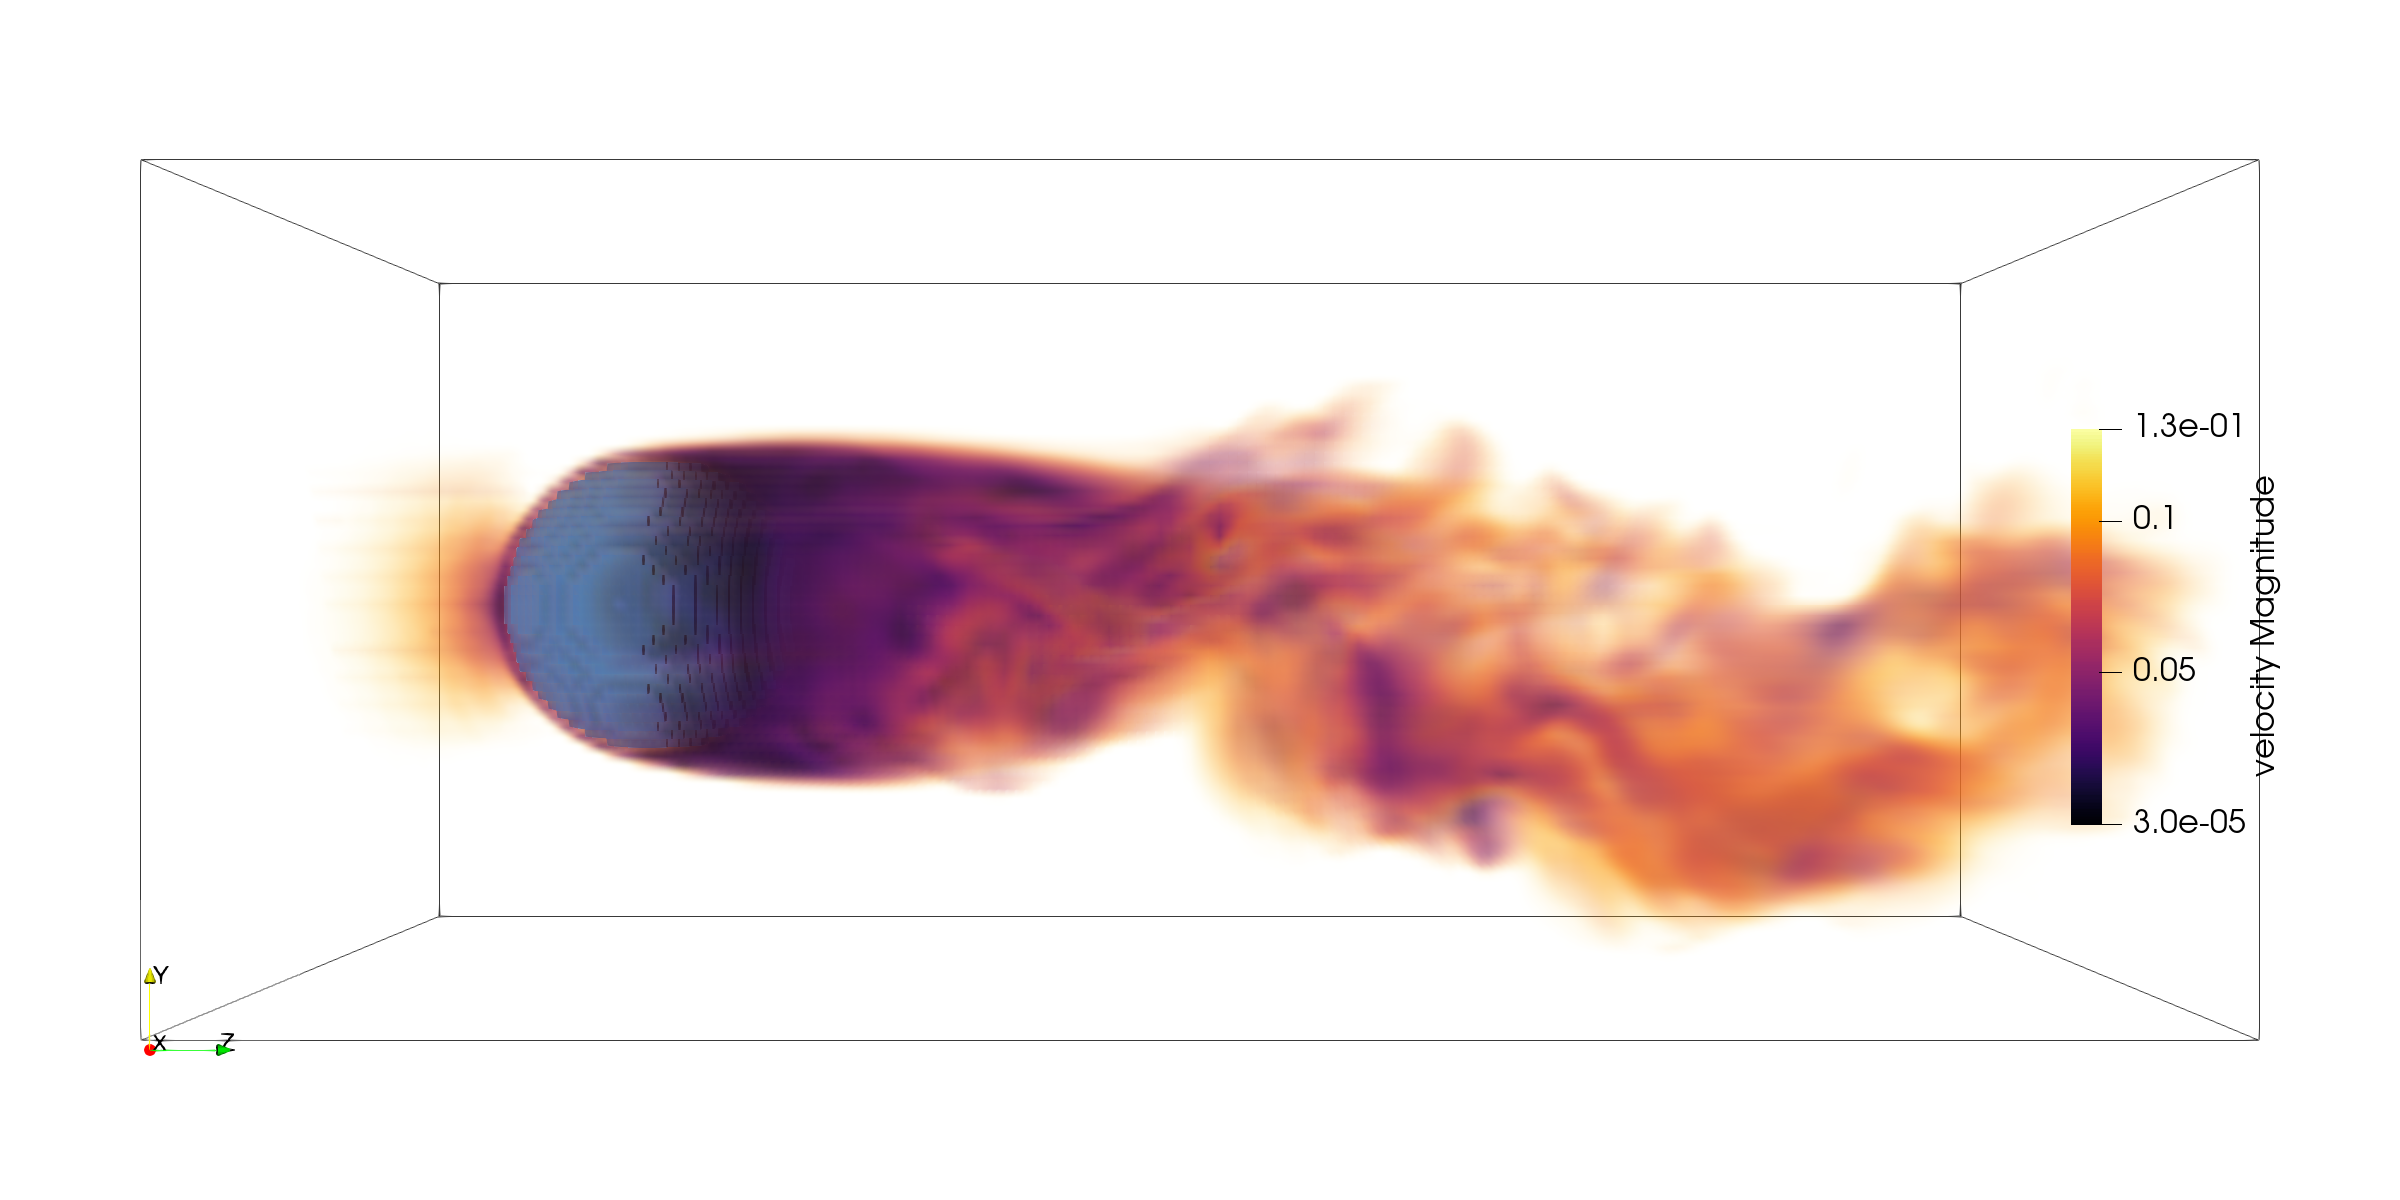
\includegraphics[width=\linewidth]{purple_render.png}
  \end{center}
\end{frame}
\placelogotrue


%%%
%%% cm_lbm slides
%%%

%\placelogofalse
\begin{frame}{Introduction}
\begin{columns}
\column{0.58\linewidth}
\centering
\begin{outline}
  \1 LBM is a framework for numerically modeling Fluid dynamics
  \1 Historically, not great for turbulence
  \1 New collision operators like CM-MRT improve this
  \1 Adoption for graphics research \cite{Li2020, Li2024, Lyu2021}
\end{outline}

\column{0.38\linewidth}
\begin{center}
\centering
\shadowimage[width=2.5cm]{li2020_image.png}

\shadowimage[width=2.5cm]{lyu2021_image.png} 
\end{center}
\end{columns}
\end{frame}
\placelogotrue

\placelogofalse
\begin{frame}{Results}
  \begin{center}
  \centering
  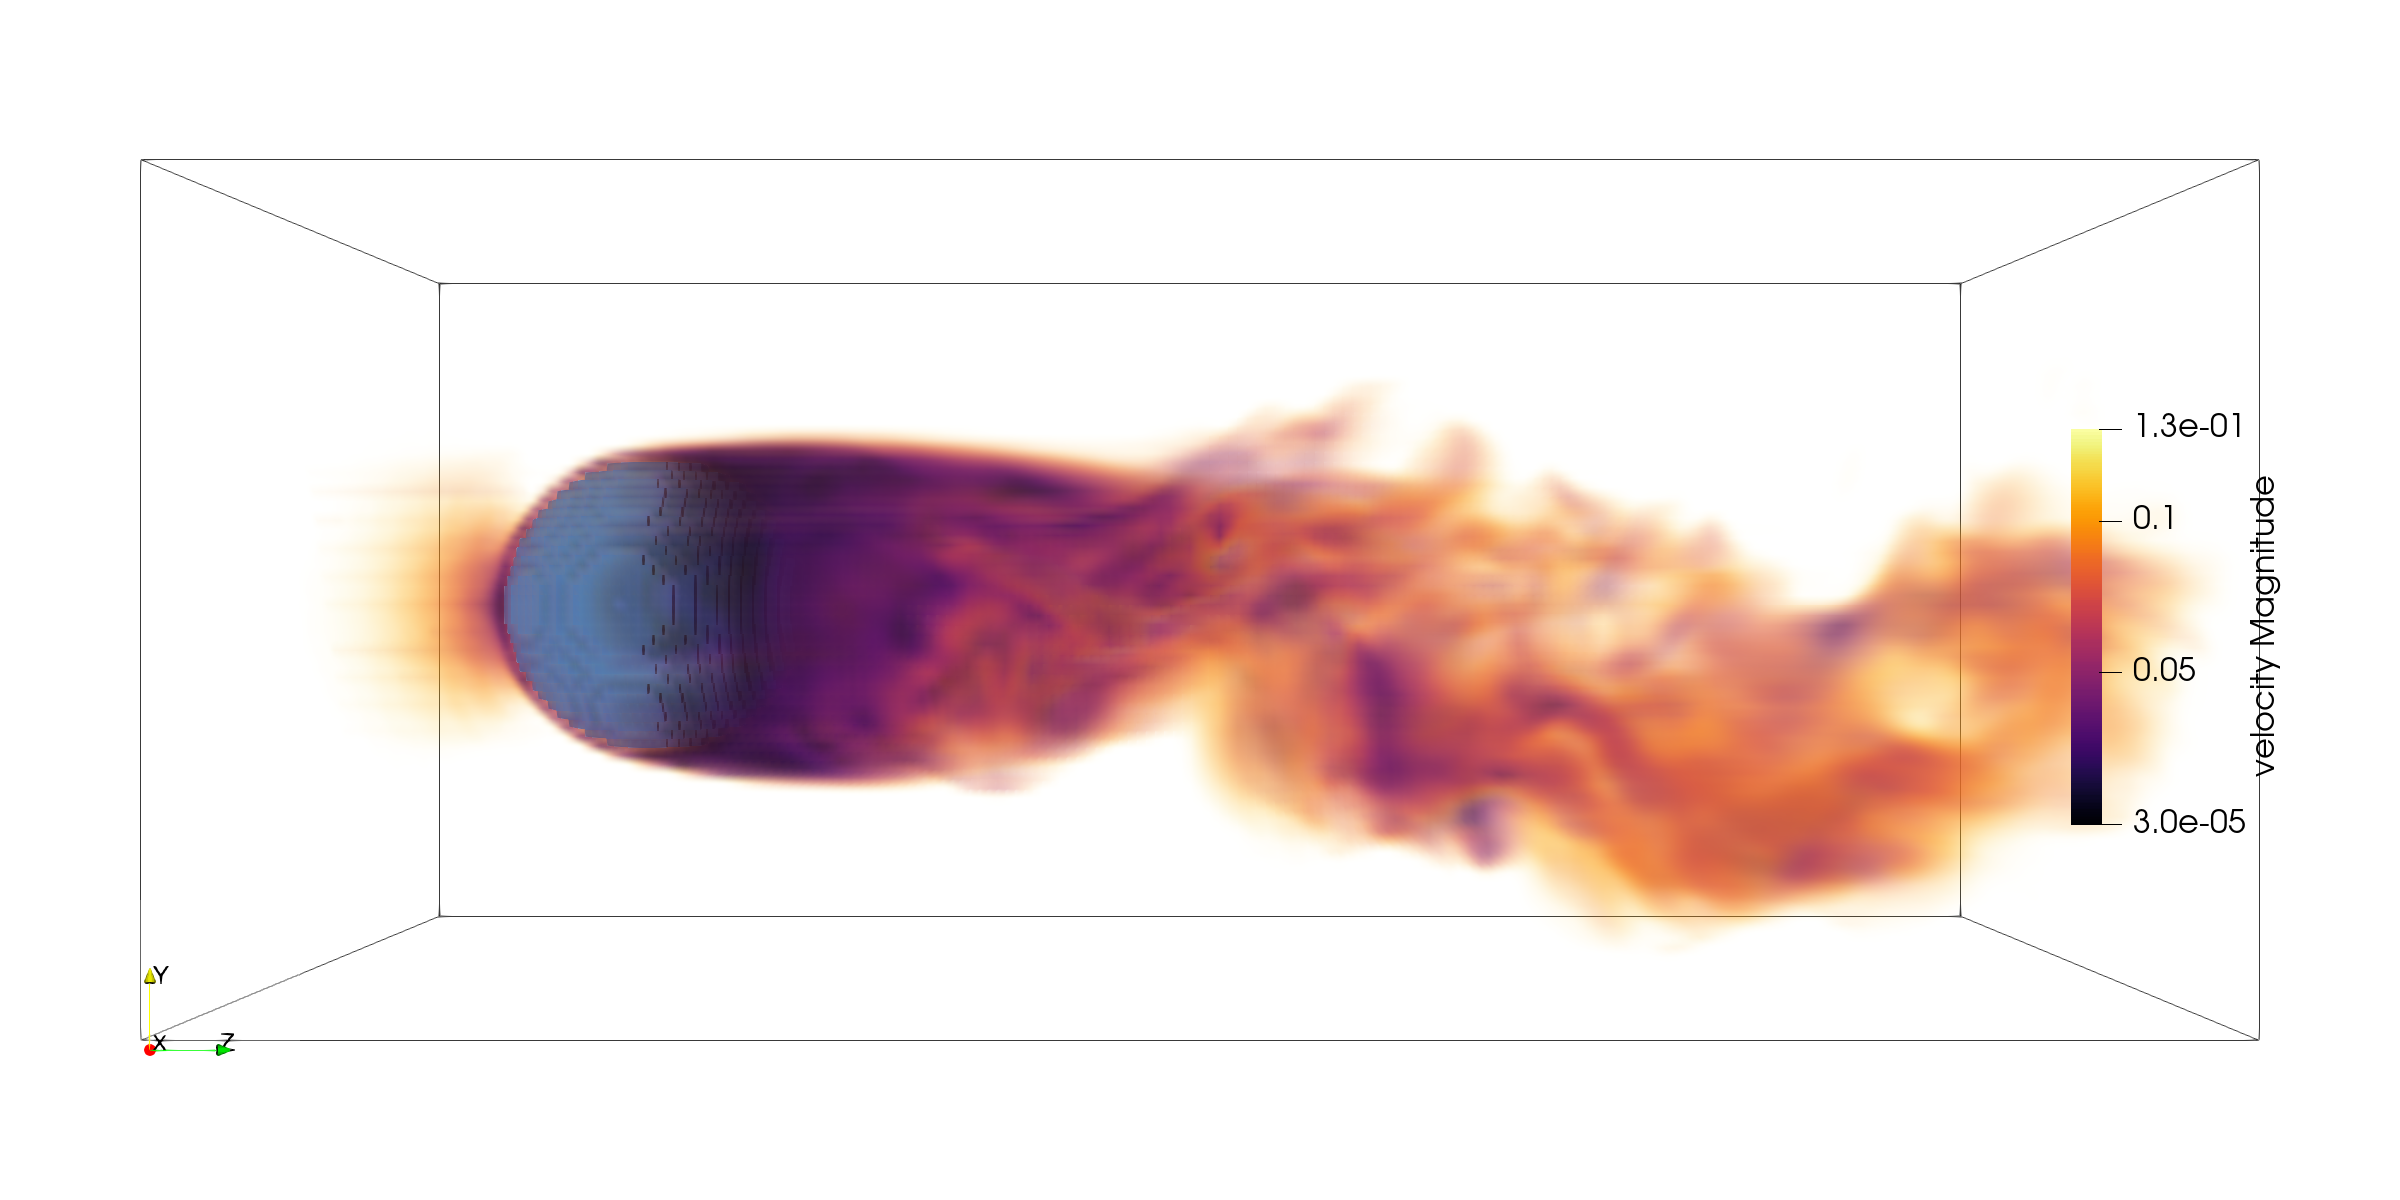
\includegraphics[width=\linewidth]{purple_render.png}
  \end{center}
\end{frame}
\placelogotrue


%\begin{frame}{Paraview + VTK}
\begin{center}
\centering
\includegraphics[width=0.7\linewidth]{example_1_paraview.png}
\end{center}
\blfootnote{\url{https://www.paraview.org}}
\blfootnote{\url{https://vtk.org}}
\end{frame}

\begin{frame}{Architecture}
  \begin{center}
  \centering
  \includegraphics[width=0.7\linewidth]{workflow.png}
  \end{center}
  \blfootnote{\url{https://github.com/SallySoul/cm_lbm}}
\end{frame}


%\placelogofalse
\begin{frame}{Classic CFD}
\begin{columns}
\column{0.48\linewidth}
\begin{outline}
\1 Discretize space into control Volumes 
\1 Solve for macroscopic fluid values
\1 Common to require global solve for pressure term
\end{outline}

\column{0.48\linewidth}
\centering
\begin{center}
\textbf{Conservation of Mass}
\begin{align*}
  \frac{\partial \rho}{\partial t} + \nabla \cdot (\rho \bm{u}) &= 0 \\
\end{align*}
\textbf{Conservation of Momentum}
\begin{align*}
\frac{\partial}{\partial t} (\rho \bm{u}) 
+ \nabla \cdot (\rho \bm{u} \times \bm{u}) &= 
- \nabla \bm{p} + \nabla \cdot \sigma
\end{align*}
  \includegraphics[width=0.8\linewidth]{FVM.png}
\end{center}
\placelogotrue

\end{columns}
\blfootnote{Figure from \href{https://www.researchgate.net/figure/Schematic-representation-of-an-FVM-model-FVM-finite-volume-method_fig5_347307910}{ResearchGate}}
\end{frame}

\placelogofalse
\begin{frame}{Lattice Boltzmann method (LBM): Discretization}
\begin{columns}
\column{0.58\linewidth}
\begin{outline}
\1 Model microscopic particles
\1 Recover macroscopic properties
\1 $D$ dimensional grid of points $x$
\2 Particle position distribution
\1 $Q$ dimensional ``lattice'' at each point
\2 Particle velocity distribution $f(x, \xi, t)$
\2 Directions $c_i$
\textit{streaming} and \textit{collision}
\end{outline}

\column{0.38\linewidth}
\centering
\begin{center}
  \includegraphics[width=0.9\linewidth]{lattice_figure.png}
  (a) D2Q9 (b) D3Q27
\end{center}
\end{columns}
\begin{align*}
  c_i &= \left\{
  \begin{array}{l l}
  (0, 0, 0) & i = 0\\
  (\pm 1, 0, 0), (0, \pm 1, 0), (0, 0, \pm) & i = 1,\ldots, 6\\
  (\pm 1, \pm 1, 0), (\pm 1, 0, \pm 1), (0, \pm 1, \pm 1)
                                            & i = 7, \ldots, 18 \\
  (\pm 1, \pm 1, \pm 1) & i = 19, \ldots, 26
  \end{array}
  \right.
\end{align*}
\blfootnote{Figure from \cite{Li2020}}
\end{frame}
\placelogotrue


\placelogofalse
\begin{frame}{LBM Theory Primer}
\begin{columns}
\column{0.48\linewidth}
\begin{outline}
\1 Lattice Boltzmann equation
\1 $f(x, t)$ approximates $\xi$
\1 Hermite Polynomial Basis \cite{De2019}
\2 Quadrature Rule with $c_i$.
\1 Collision operator, $\Omega$
\2 Relax towards equilibrium $f_{eq}$
\1 Moments of $f$ are macroscopic quantities 
\1 Advance time with two operators, 
\textit{streaming} and \textit{collision}
\end{outline}
\column{0.48\linewidth}
\centering
\begin{center}
  \begin{align*}
  \partial_t f(x, \xi, t)  + \xi \cdot \nabla f(x, \xi, t) = \Omega (f)
  \end{align*}

  \begin{align*}
  \rho(x, t) &= \sum_{i = 0}^{Q - 1} f_i(x, t) \\
  \rho(x,t)u(x,t) &= \sum_{i = 0}^{Q - 1}c_i f_i(x, t)
  \end{align*}
\end{center}
\end{columns}
\blfootnote{Figure from \cite{Li2020}}
\end{frame}
\placelogotrue

\begin{frame}{Streaming}
\begin{columns}
\column{0.48\linewidth}
\begin{outline}
\1 Non-local operator (Transport)
\1 Particles stream to next point in grid 
\1 Information travels at speed of sound!
\end{outline}
\begin{align*}
  f^{*}_i(x, t) &= f_i(x - c_i, t) 
\end{align*}
\column{0.48\linewidth}
\centering
  \begin{center}
    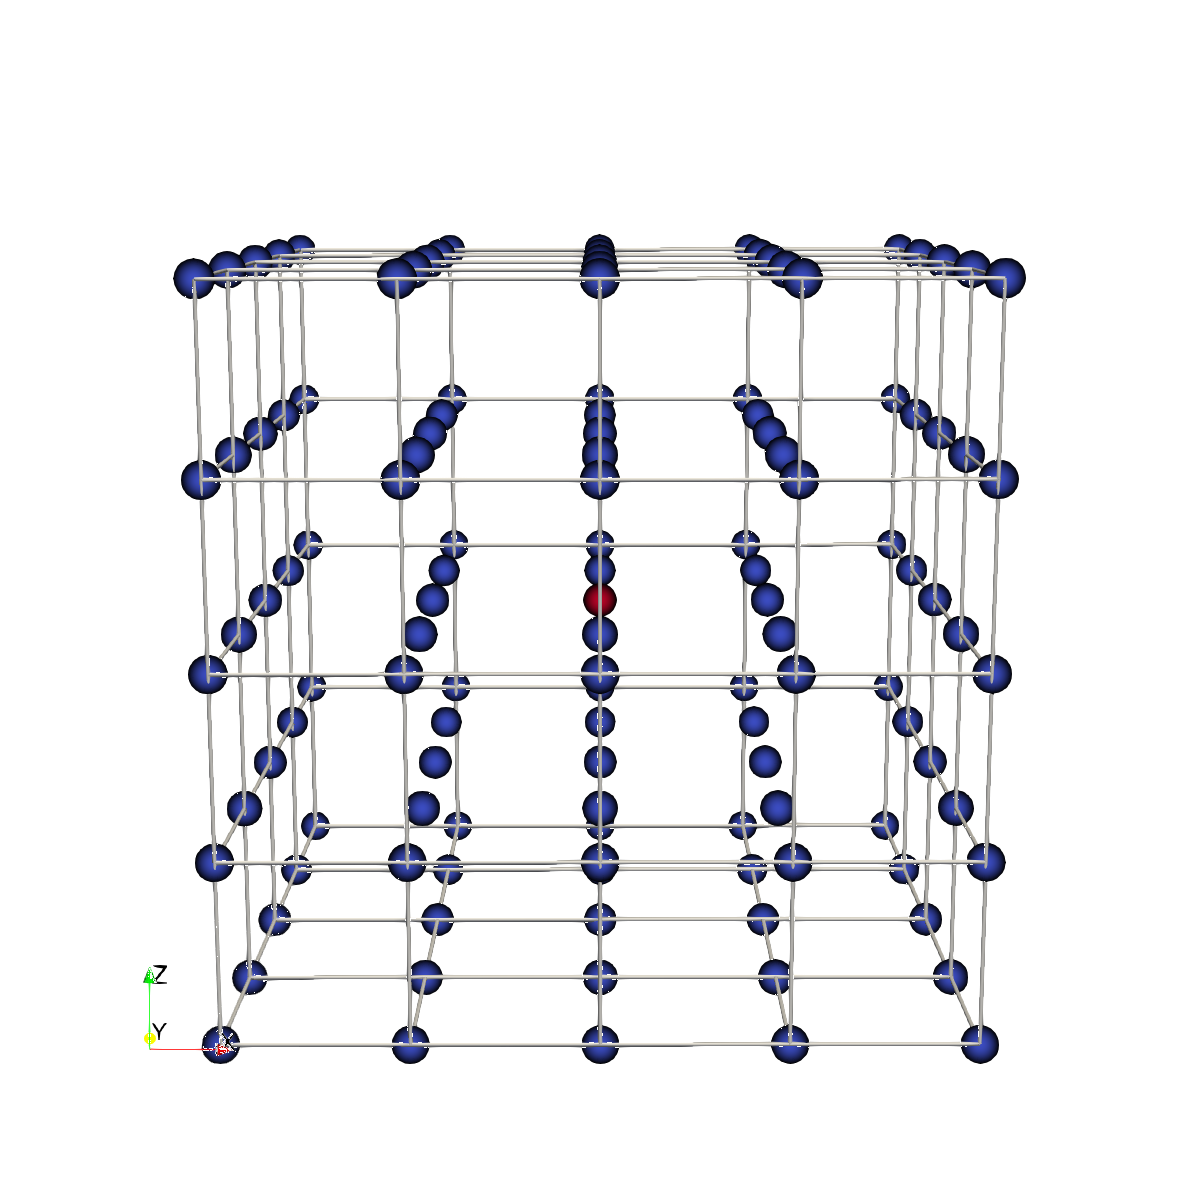
\includegraphics[width=0.4\linewidth]{stream_0.png}
    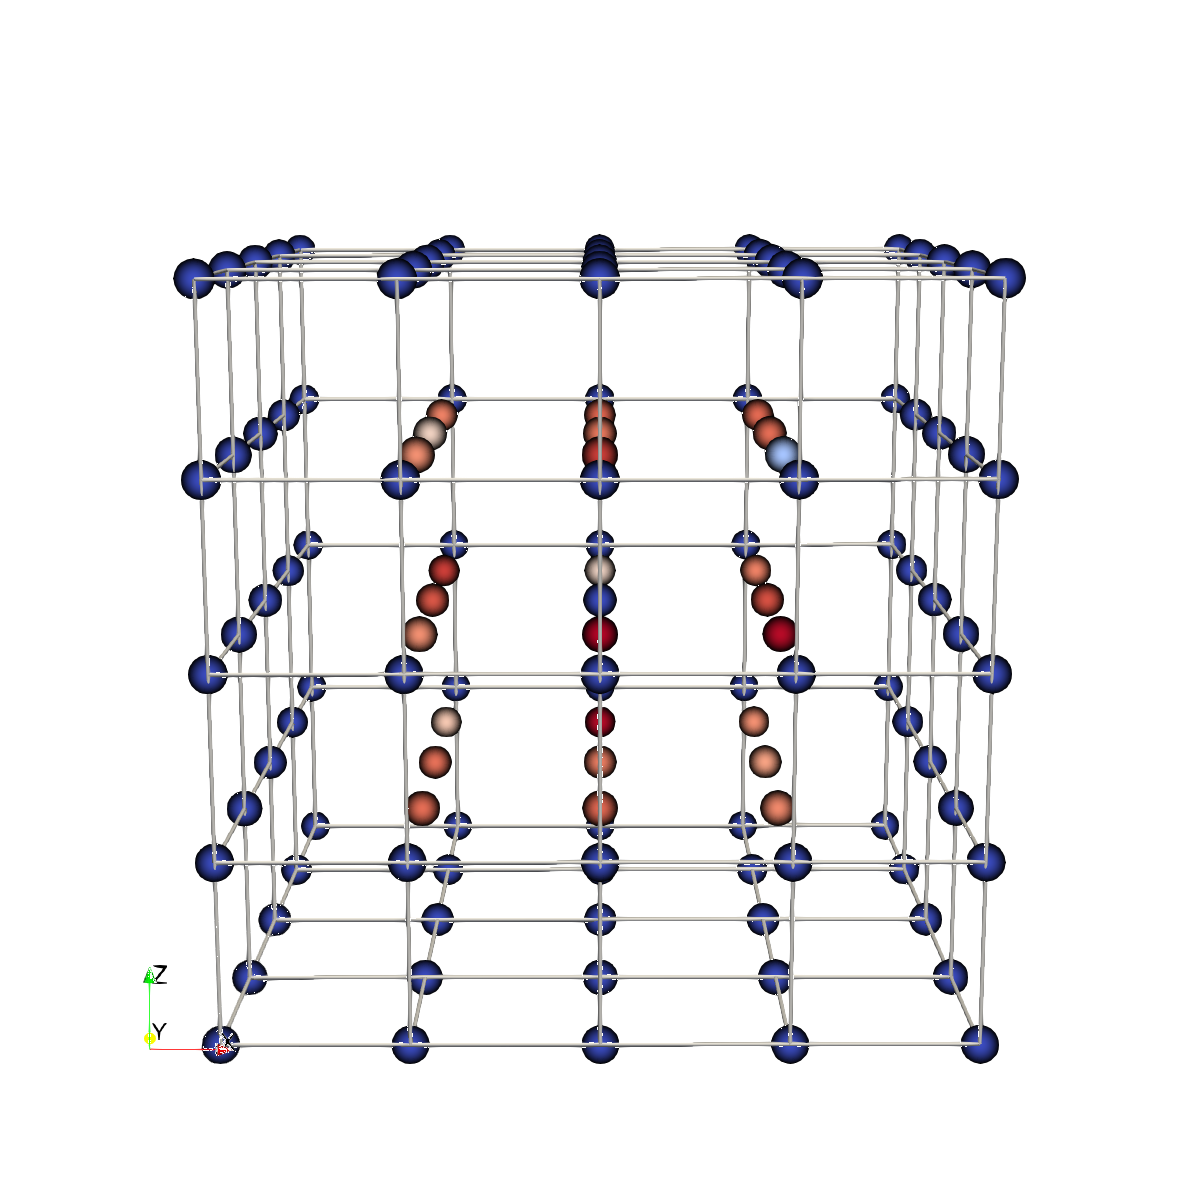
\includegraphics[width=0.4\linewidth]{stream_1.png}

    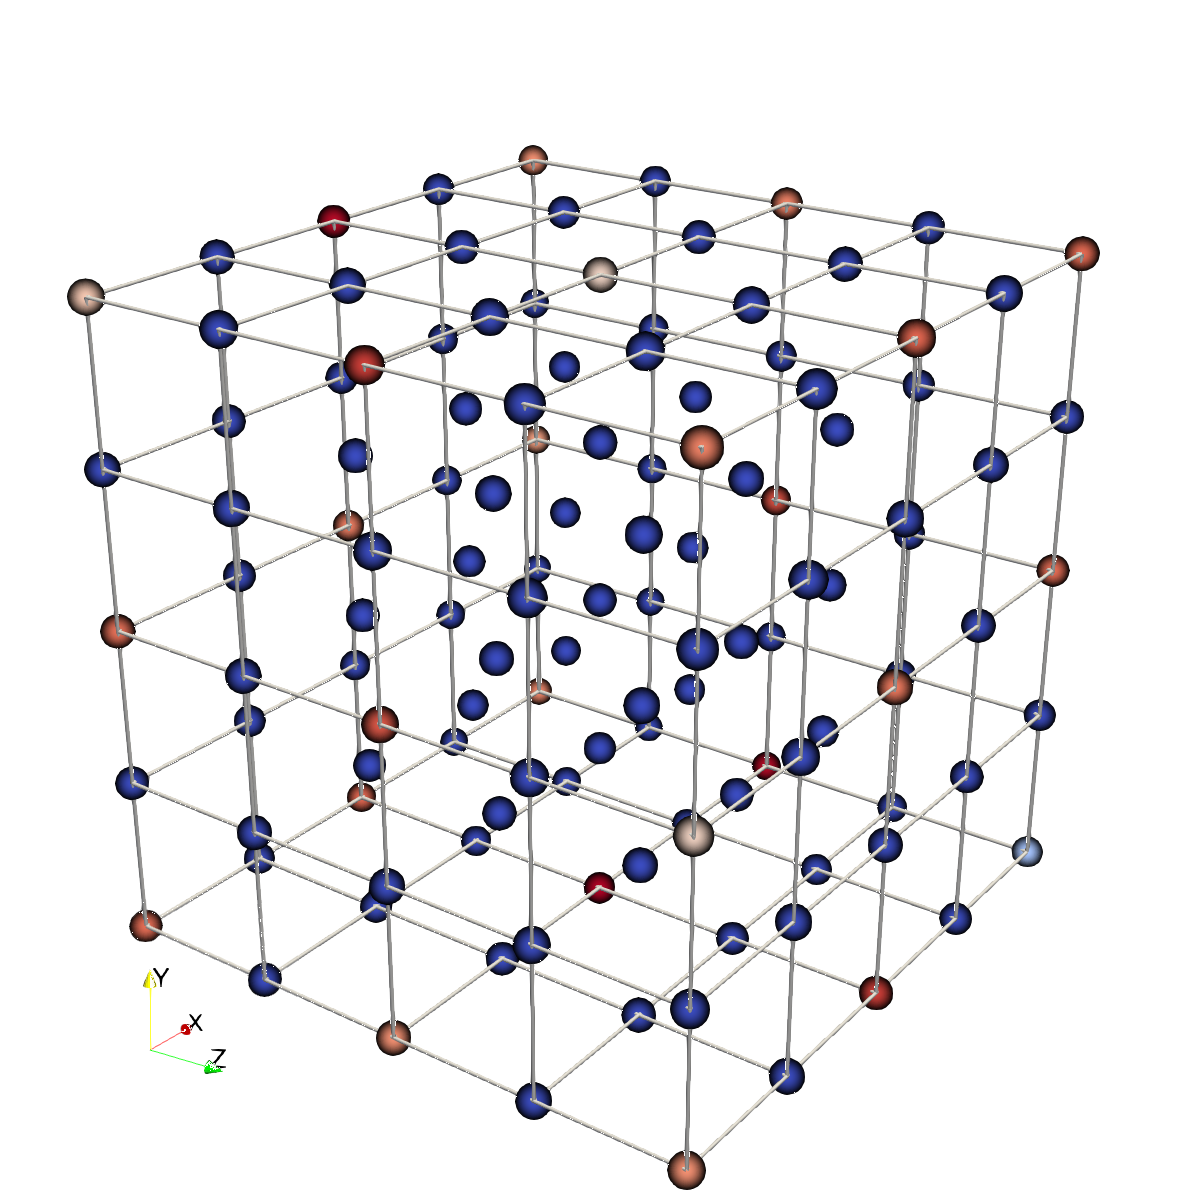
\includegraphics[width=0.6\linewidth]{stream_2.png}
  \end{center}
\end{columns}
\end{frame}




%\begin{frame}{Collision (BGK)}
\begin{columns}
\column{0.48\linewidth}
\begin{outline}
\1 Collision is local
\1 Relax distributions towards equilibrium
\1 BGK is standard collision operator
\2 Relaxes all distributions at constant rate
\1 First order approximation
\end{outline}
\column{0.48\linewidth}
\begin{center}
\begin{align*}
    \text{BGK}(f) &= \frac{1}{\tau} (f_{\text{eq}} - f)
\end{align*}
\end{center}
\end{columns}
\vspace{1cm}
\begin{align*}
   f_{\text{eq}} &= w_i \rho \left(
1 + 3 c_i \cdot u  + \frac{9 (c_i \cdot u)^2}{2}
- \frac{3 (u \cdot u)^2}{2}\right) \\
\end{align*}
\end{frame}

\begin{frame}{Multiple Relaxation Time (MRT)}
\begin{columns}
\column{0.48\linewidth}
\begin{outline}
\1 $M$ transforms $f$ into moment space
\1 $26$ of them!
\1 Relax moments separately
\1 $M^{-1}$ transforms result back to distribution
\end{outline}
\column{0.48\linewidth}
\begin{center}
\begin{align*}
m_{0,j} &= \{  1 \},\\
m_{1,j} &= \{  c_{j,x} \}, \\
m_{18,j} &= \{ c_{j,x}^2 c_{j,y}^2 + c_{j,x}^2 c_{j,z}^2 - c_{j,y}^2 c_{j,z}^2 \}, \\
m_{19,j} &= \{ c_{j,x}^2 c_{j,y}^2 - c_{j,x}^2 c_{j,z}^2 \},\\
m_{26,j} &= \{ c_{j,x}^2 c_{j,y}^2 c_{j,z}^2 \},\\
\end{align*}
\end{center}
\end{columns}
\begin{center}
  \begin{align*}
\text{MRT}(f) &= M^{-1} \cdot R \cdot M(f_{\text{eq}} - f)
  \end{align*}
\end{center}
\end{frame}

\begin{frame}{Relaxation Rates, pt 1}
\begin{columns}
\column{0.48\linewidth}
\begin{outline}
\1 Independent relaxation rates for each moment
\1 Zeroth moment, density, should be conserved.
\1 Next three are momentum, $r_i = 2$ is common
\1 Next six moments are related to momentum flux
\2 Relaxation rate is related to viscosity, $v$ 
\end{outline}
\column{0.48\linewidth}
\begin{center}
\begin{align*}
  R &= \left[\begin{array}{c c c c}
  r_0 & 0 & \cdots & 0 \\
  0 & r_1 & \cdots & 0 \\
  \vdots & & & \vdots \\
  0 & & \cdots & r_{26} \\
  \end{array}\right] \\
  r_0 &= 0, \\
  r_i &= 2, \text{ for } i = 1, 2, 3 \\
  r_i &= (3v + 1/2)^{-1}, \text{ for } i = 4,\cdots,9
\end{align*}
\end{center}
\end{columns}
\end{frame}

\begin{frame}{Relaxation Rates, pt 2}
\begin{columns}
\column{0.48\linewidth}
\begin{outline}
\1 Higher-order relaxation rates are an area of active research
\1 \cite{Li2020} Describes an adaptive approach
\1 I implemented fixed rates as described in \cite{Li2018}.
\end{outline}
\column{0.48\linewidth}
\begin{center}
\begin{align*}
  R &= \left[\begin{array}{c c c c}
  r_0 & 0 & \cdots & 0 \\
  0 & r_1 & \cdots & 0 \\
  \vdots & & & \vdots \\
  0 & & \cdots & r_{26} \\
  \end{array}\right] \\
  r_i &= (3v_i + 1 / 2)^{-1}\\
  v_i &= 0.005, \text{ for } i = 9,\ldots, 16 \\
  v_i &= 0.007, \text{ for } i = 17, \ldots, 22 \\
  v_i &= 0.009, \text{ for } i = 26 
\end{align*}
\end{center}
\end{columns}
\end{frame}


\placelogofalse
\begin{frame}{Central Moment MRT (CM-MRT)}
\begin{columns}
\column{0.48\linewidth}
\begin{outline}
\1 MRT violates Galilean invariance 
\2 $u$ changes collision outcome
\1 Center Moments on $u$ \cite{De2017}
\1 $\bar{m}_{\rho} = M_u f_{eq}(u, \rho)$
\2 Equilibrium in CM space
\2 Only depends on $\rho$!
\end{outline}
\column{0.48\linewidth}
\begin{center}
\begin{align*}
\bar{c}_j &= c_j - u \\
m_{0,j} &= \{  1 \},\\
m_{1,j} &= \{  \bar{c}_{j,x} \}, \\
m_{18,j} &= \{ \bar{c}_{j,x}^2 \bar{c}_{j,y}^2 + \bar{c}_{j,x}^2 \bar{c}_{j,z}^2 - \bar{c}_{j,y}^2 \bar{c}_{j,z}^2 \}, \\
m_{19,j} &= \{ \bar{c}_{j,x}^2 \bar{c}_{j,y}^2 - \bar{c}_{j,x}^2 \bar{c}_{j,z}^2 \},\\
m_{26,j} &= \{ \bar{c}_{j,x}^2 \bar{c}_{j,y}^2 \bar{c}_{j,z}^2 \},\\
\end{align*}
\end{center}
\end{columns}
\begin{center}
  \begin{align*}
\text{CM-MRT}_{u,\rho}(f) &= M_u^{-1} \cdot R \cdot (\bar{m}_{\rho} - M_u f)
\end{align*}
\end{center}
\end{frame}
\placelogotrue

\placelogofalse
\begin{frame}{Central Moment MRT (CM-MRT)}
\begin{columns}
\column{0.48\linewidth}
\begin{outline}
\1 MRT violates Galilean invariance 
\1 Center Moments on $u$ \cite{De2017}
\1 $f_{\text{eq}}$ only depends on $\rho$ in CM space
\end{outline}
\column{0.48\linewidth}
\begin{center}
\begin{align*}
\bar{c}_j &= c_j - u \\
m_{0,j} &= \{  1 \},\\
m_{1,j} &= \{  \bar{c}_{j,x} \}, \\
m_{18,j} &= \{ \bar{c}_{j,x}^2 \bar{c}_{j,y}^2 + \bar{c}_{j,x}^2 \bar{c}_{j,z}^2 - \bar{c}_{j,y}^2 \bar{c}_{j,z}^2 \}, \\
m_{19,j} &= \{ \bar{c}_{j,x}^2 \bar{c}_{j,y}^2 - \bar{c}_{j,x}^2 \bar{c}_{j,z}^2 \},\\
m_{26,j} &= \{ \bar{c}_{j,x}^2 \bar{c}_{j,y}^2 \bar{c}_{j,z}^2 \},\\
\end{align*}
\end{center}
\end{columns}
\begin{center}
  \begin{align*}
\text{CM-MRT}_{u,\rho}(f) &= M_u^{-1} \cdot R \cdot (\bar{m}_{\rho} - M_u f)
\end{align*}
\end{center}
\end{frame}
\placelogotrue


%\begin{frame}{Code Example: SymPy}
  \begin{center}
  \begin{align*}
  f^{*}_i = f_i + \Omega_i(f, \rho, u).
  \end{align*}
  \shadowimage[width=0.46\linewidth]{bgk_python_code.png}
  \shadowimage[width=0.46\linewidth]{python_code.png}
  \begin{outline}
    \1 Using SymPy was inspired by \cite{Hennig2023}
    \1 Looks like a compiler
  \end{outline}
  \end{center}
\end{frame}

\begin{frame}{Code Example: Shader}
  \begin{center}
  \shadowimage[width=0.6\linewidth]{shader_code.png}
  \end{center}
  \begin{outline}
    \1 $\approx 5$kb for moments shader
    \1 $1.1$mb for CM-MRT shader
    \1 Cheap to compute
    \1 Challenging to debug
  \end{outline}
\end{frame}

\begin{frame}{Code Example: Rust}
  \begin{center}
  \shadowimage[width=0.6\linewidth]{rust_code.png}
  \end{center}
  \begin{outline} 
    \1 With formatting, $\approx 45$k lines
    \1 Easier to test and debug
    \1 Tricky parts match shader exactly
\end{outline}
\end{frame}





 % Graphicsfinal conclusion
%\begin{frame}{Graphics Final Conclusion}
  \begin{outline}
    \1 How are we feeling about the paper title?
    \2 MRT Lattice Boltzmann methods?
    \2 Code generation using \lstinline{sympy}?
    \1 LBM + \lstinline{sympy}
      \2 \href{http://literatelb.org}{``A Literate Lattice Boltzmann Code''} \cite{web:literatelbm}
  \end{outline}
  \begin{center}
    \includegraphics[width=0.8\linewidth]{title_header.png}
  \end{center}
\end{frame}


%%
%% Paper Slides
%%

% Background Projects
%\begin{frame}{Paper Context}
  \begin{outline}
    \1 Collaborative HPC work at German University
    \1 \href{https://www.fau.eu}{Fridrich-Alexander-Universit{\"a}t}
    \1 HPC stuff? 
  \end{outline}
\end{frame}

%\placelogofalse
\begin{frame}{waLBerla}
\begin{columns}
\column{0.48\linewidth}
\begin{outline}
  \1 waLBerla framework 
  \2 Introduced in \cite{Bauer2021} (2021)
  \2 HPC-scale simulations
  \2 Stencil problems specifically
  \2 Bring your Compute Kernels
  \1 Provides:
  \2 Multi-node domain partitioning
  \2 Communication patterns 
  \2 Checkpoints
\end{outline}
\column{0.48\linewidth}
\begin{center}
  \shadowimage[width=0.8\linewidth]{juwels.png}
  \vspace{0.5cm}
  \includegraphics[width=0.8\linewidth]{walberla_partition.png}
  \vspace{0.5cm}
  \includegraphics[width=0.8\linewidth]{walberla_examples.png}
\end{center} 
\end{columns}
\blfootnote{From \href{t}{TODO}, \cite{Bauer2021}}
\end{frame}
\placelogotrue


%\begin{frame}{\lstinline{pystencils}}
\begin{columns}
  \column{0.48\linewidth}
  \begin{outline}
  \1 Introduced in 2019 \cite{Bauer2019}
  \1 Stencil Compiler 
  \2 \lstinline{sympy}

  \2 Generates optimized compute Kernels
  \2 Introduced in \cite{Bauer2021} (2020)
  \end{outline}

  \column{0.48\linewidth}
  \centering
  \begin{center}
    \includegraphics[width=0.2\linewidth]{pystencils_logo.png}
  \end{center}
\end{columns}
\end{frame}

%\begin{frame}{\lstinline{lbmpy}}
  \begin{columns}
  \column{0.48\linewidth}
  \begin{outline}
  \1 Python package for LBM
  \2 Introduced in \cite{Bauer2021} (2020)
  \end{outline}

  \column{0.48\linewidth}
  \centering
  \begin{center}
    \includegraphics[width=0.2\linewidth]{lbmpy_logo.png}
  \end{center}
\end{columns}
\end{frame}


% Paper intro
%\placelogofalse
\begin{frame}{Introduction}
\begin{columns}
\column{0.48\linewidth}
\begin{outline}
  \1 Presenting \cite{Hennig2023} (2023)
  \1 Re-architecture of {lbmpy}
  \2 Zero-centered Storage
  \2 Central Moment (CM)
  \2 Cumulants (K)
  \2 Support more generic governing eqns
  \1 Minimizes arithmetic operations for CM and K methods
  \1 Demonstrate small relative cost compared to SRT
\end{outline}
\column{0.48\linewidth}
\begin{center}
  \shadowimage[width=0.46\linewidth]{hennig_paper.png}

  \includegraphics[width=0.28\linewidth]{frederik_hennig.jpg}
  \includegraphics[width=0.28\linewidth]{markus_holzer.jpg}

  \includegraphics[width=0.28\linewidth]{ulrich_rude.jpg}
\end{center} 
\end{columns}
\end{frame}
\placelogotrue



% Zero-centered
\begin{frame}{Zero-centered Storage}
TODO
\end{frame}


% TODO Simplication Passes 
\begin{frame}{Simplification Passes}
  \begin{columns}
  \column{0.58\linewidth}
  \begin{outline}
    \1 Conserved Quantity Rewriting
    \2 Use moments instead of $\rho, \bm{u}$
    \1 Propagation of Logarithms
    \2 Relevant for Cumulants
    \1 Common Subexpression Elimination (CSE)
    \2 Make new assignments for them
    \1 Expression Propagation
    \2 For assignments with constant RHS
    \2 Copy into use-sites
    \1 Unused Subexpression Elimination
    \2 Remove unused assignments
  \end{outline}
  \column{0.38\linewidth}
  \centering
  \begin{center}
  \begin{align*}
    \kappa_{000} &= \rho \\
    \kappa_{100} &= -F_x / 2 \\
    \kappa_{000}^{*} &= \kappa_{000} \\
    \kappa_{100}^{*} &= \kappa_{100} + F_x \\
    m^{*}_{10|0} &= \kappa^{*}_{000} \bm{u}_x + \kappa_{100}^{*}
  \end{align*}
  To
  \begin{align*}
  m^{*}_{10|0} &= \rho \bm{u}_x + F_x / 2 
  \end{align*}
\end{center}
\end{columns}
\end{frame}

\begin{frame}{Moment Transform, pt. 1}
\begin{columns}
\column{0.48\linewidth}
\begin{outline}
  \1 Transform populations to Raw Moments ($Mf$)
  \1 Use Chimera transform to compute moments    
  \2 Introduced in \cite{Geier2015}
  \1 More efficient than Matrix transform
  \1 Inverse uses trick to split populations \\
  $f^{*}_i = f^{+}_i + f^{-}_i, \ f^{*}_{\bar{i}} = f_i^{+} - f^{-}_i$
\end{outline}

\column{0.48\linewidth}

\centering
\begin{center}
\begin{align*}
  m_{xy|\gamma} &:= \sum_{z \in \{-1, 0, 1\}} f_{xyz} \cdot z^{\gamma} \\ 
  m_{x|\beta\gamma} &:= \sum_{y \in \{-1, 0, 1\}} m_{xy|\gamma} \cdot y^{\beta} \\ 
  m_{\alpha\beta\gamma} &:= \sum_{x \in \{-1, 0, 1\}} m_{x|\beta\gamma} \cdot x^{\alpha} \\ 
\end{align*}
\end{center}
\end{columns}
\end{frame}

\begin{frame}{Moment Transform, pt. 2}
\begin{columns}
\column{0.48\linewidth}
\begin{outline}
  \1 To compute central moments
  \1 First compute raw moments $m_{\alpha\beta\gamma}$
  \1 Then transform them to central moments $\kappa_{\alpha\beta\gamma}$
\end{outline}

\column{0.48\linewidth}

\centering
\begin{center}
\begin{align*}
  \kappa_{ab|\gamma} &:= 
  \sum_{c = 0}^{\gamma} \binom{\gamma}{c} (-u_z)^{\gamma - c} m_{a b c} \\
  \kappa_{a|\beta\gamma} &:= 
  \sum_{c = 0}^{\gamma} \binom{\gamma}{c} (-u_z)^{\gamma - c} m_{a b c} \\
\end{align*}
\end{center}
\end{columns}

  \begin{align*}
    \kappa_{\alpha\beta\gamma} = 
    \sum_{a, b, c = 0}^{\alpha\beta\gamma} 
    \binom{\alpha}{a} \binom{\beta}{b} \binom{\gamma}{c} 
    (-u_x)^{\alpha - a}(-u_y)^{\beta - b} (-u_z)^{\gamma - c} m_{a b c}
  \end{align*}


\end{frame}



%% "Operation Count"
% rg '\+|\*|\-' cm_lbm_generated/src/shader_ops/cm_mrt.rs -o  | wc -l
\begin{frame}{Symbolic Simplification Results}
  \centering
  \begin{center}
    \includegraphics[width=0.8\linewidth]{arith_table.png}
  \end{center}
  For reference, my had \textsc{CM} implementation (slight over estimate) $220,702$ arithmetic operations.
  \blfootnote{From \cite{Hennig2023}}
\end{frame}






%\section{Conclusion}

I have presented our LBM implementation, 
\lstinline{cm_lbm}. I have explained the background theory to 
explain its operation, 
as well as how it relates to the latest research in this area.
I also outlined future work that would bring this project
closer to the true state of the art.
This project mostly satisfies the goals laid out in my proposal,
but came up short in a few areas, notably rendering and 
fluid solid coupling.
Nonetheless, I feel that this has opened up 
several research avenues for me to pursue.




% Eh
% \begin{frame}
  \begin{outline}
   \1 \cite{Yu2025Filter}
  \end{outline}
\end{frame}


\begin{frame}[allowframebreaks]{References}
    \tiny
    \printbibliography
\end{frame}

\end{document}


